\documentclass[runningheads]{llncs}

% ---------------------------------------------------------------
% ECCV package
\usepackage[review,year=2026,ID=13150]{eccv}
\usepackage{eccvabbrv}

% ---------------------------------------------------------------
% Common packages
\usepackage[table,xcdraw]{xcolor}
\usepackage{graphicx}
\usepackage{booktabs}
\usepackage{amsmath}
\usepackage{amssymb}
\usepackage{multirow}
\usepackage{array}
\usepackage[accsupp]{axessibility}
\usepackage{hyperref}

\newcolumntype{C}[1]{>{\centering\arraybackslash}m{#1}}
\definecolor{groupbg}{RGB}{226,236,248}
\definecolor{groupfg}{RGB}{44,62,92}

\begin{document}

\title{Following the Flow: Advection-Consistent Modeling for Event-based Small Object Detection\\[0.5ex]
Supplementary Material}

\titlerunning{Supplementary Material}
\author{Anonymous Authors}
\authorrunning{Anonymous Authors}
\institute{ECCV 2026 Submission ID 13150}

\maketitle

\section{Additional Related Work}

Event-based learning has gradually moved beyond using asynchronous streams only as regular tensors or recurrent states for downstream models \cite{gehrig2019end,gehrig2023recurrent}.
More recent studies begin to examine the representation itself.
Zubi\'c \etal show that dense event representations can be explicitly ranked with Gromov-Wasserstein discrepancy for downstream tasks \cite{zubic2023chaos}, and later introduce state-space models for event cameras to replace conventional recurrence with learned temporal dynamics \cite{zubic2024state}. 
Asynchronous sparse processing has also continued to develop.
Schaefer \etal update only the affected part of an evolving spatio-temporal graph in AEGNN \cite{schaefer2022aegnn}, Messikommer \etal convert synchronous event models into asynchronous sparse ones while preserving identical outputs \cite{messikommer2020asyncsparse}, and Li \etal further couple frames and events in a unified asynchronous graph representation \cite{li2025asynchronous}. 
On the detector side, Torbunov \etal adapt image detectors to event-based vision in latent space rather than redesigning the detector from scratch \cite{torbunov2025evrt}. 
Across these developments, the emphasis remains on how event streams are represented, updated, or transferred into downstream models. 
The formulation adopted here enters at a later stage, when weak encoded responses already exist and must remain coherent over time.

Motion-guided event modeling has likewise developed beyond early event warping. 
Gallego \etal formulate event alignment through contrast maximization under a motion model, while Benosman \etal relate this motion-compensation view to event-based visual flow estimation \cite{gallego2018unifying,benosman2013event}. 
Gallego \etal further compare a broad family of focus-based losses and analyze how different objectives affect motion-related estimation \cite{gallego2019focus}. 
Motion compensation has also been used more directly for motion segmentation and moving-object analysis \cite{stoffregen2019event,mitrokhin2018event}.
More recent work begins to model motion together with degradation in the data itself: Shiba \etal estimate motion and noise jointly \cite{shiba2025simultaneous}, while Yamaki \etal extend contrast-maximization-based motion segmentation to an iterative variational framework \cite{yamaki2025iterative}. 
Within this line, motion is still used mainly to align raw events, refine compensation, or define optimization targets. 
The advection-based formulation adopted here instead uses a local velocity field after encoding, where latent features are transported and weak responses are judged by whether they remain consistent under that transport.

\begin{table*}[t]
\centering
\caption{Detailed training settings of the compared methods on EV-UAV.
% The compared methods follow the configurations reported in their original papers, as our training configuration did not yield better performance for these baselines.
Baseline methods follow the configurations reported in their original papers, as alternative training configurations did not improve their performance.}
\label{tab:additional_settings}
\small
\renewcommand{\arraystretch}{1.15}
\setlength{\tabcolsep}{3pt}
\begin{tabular}{lcccccc}
\toprule
Method & Input & Optimizer & LR & Scheduler & Batch & Epochs \\
\midrule

\multicolumn{7}{l}{\textcolor{groupfg}{\textit{Frame-based methods}}} \\
SSD & \multirow{4}{*}{50ms/frame} & SGD & 1e-3 & Step & 32 & 100 \\
Faster R-CNN &   & SGD & 1e-3 & Step & 8  & 100 \\
DETR         &   & AdamW  & 1e-4   & Step & 8  & 150 \\
YOLOv10-S    &      & SGD & 1e-2 & Linear & 16 & 100 \\
\midrule

\multicolumn{7}{l}{\textcolor{groupfg}{\textit{SNN-based methods}}} \\
EMS-YOLO     & \multirow{2}{*}{2.5s/5 slice}  & SGD & 1e-2 & Cosine & 32 & 100 \\
SpikeYOLO    &   & SGD & 1e-2 & Cosine & 20 & 50 \\
GET          & 50ms/12 groups & Adam & 2e-4 & OneCycle & 8 & 50 \\
\midrule

\multicolumn{7}{l}{\textcolor{groupfg}{\textit{Voxel-based methods}}} \\
RED          & \multirow{3}{*}{50ms/10 slice volume} & Adam   & 2e-4 & Exponential & 8 & 20 \\
RVT          &  & Adam   & 2e-4 & OneCycle & 8 & 50 \\
SAST         &   & AdamW & 5e-4 & Cosine & 16 & 50 \\
\midrule

\multicolumn{7}{l}{\textcolor{groupfg}{\textit{Point-based methods}}} \\
KPConv       & \multirow{4}{*}{8s/point stream} & Momentum & 1e-2 & Step & 10 & 400 \\
RandLA-Net   &   & Adam   & 1e-2 & Exponential & 8  & 100 \\
COSeg        &   & AdamW  & 5e-5 & Cosine & 4 & 100 \\
EV-SpSegNet  &   & Adam   & 1e-2 & Linear & 8   & 50 \\
\midrule

\multicolumn{7}{l}{\textcolor{groupfg}{\textit{Ours}}} \\
PACT (ours)  & 8s/point stream & Adam & 1e-3 & StepLR & 4 & 50 \\
\bottomrule
\end{tabular}
\end{table*}

Benchmark development shows a similar difference in emphasis. 
Perot \etal introduce the 1 Mpx dataset for general event-based detection in high-resolution automotive scenes \cite{perot2020learning}.
The earlier large-scale automotive benchmark of de Tournemire \etal provides longer driving recordings but excludes targets whose bounding-box diagonal is smaller than 30 pixels \cite{detournemire2020automotive}. 
More recently, Chen \etal shift the focus to event-based tiny object detection with EV-UAV, emphasizing extremely small targets in complex anti-UAV scenarios \cite{chen2025event}. 
This setting is closer to the one considered here, where the challenge is not only whether a target can be detected, but whether weak and fragmented evidence can remain temporally continuous once event support becomes sparse and easily interrupted.

\section{Additional Experimental Settings}
For reproducibility, we further summarize the experimental settings of the compared methods on EV-UAV. Since these baselines follow different input paradigms, we configure their inputs accordingly. The resulting input formats and training configurations are reported in Table~\ref{tab:additional_settings}.

\section{Ablation on the Number of Hypotheses $K$}
We study the effect of the hypothesis number $K$ used in the A-FR module. 
This parameter determines how many perturbed transport candidates are generated around the estimated local velocity field during advection-guided propagation. 
When $K$ is too small, the candidate set cannot adequately cover motion uncertainty, making the decoder less stable when velocity estimation is unreliable in sparsely activated regions. 
As $K$ increases, the model can evaluate a broader set of transport hypotheses and better recover fragmented responses along plausible trajectory directions. 
However, an overly large $K$ also introduces redundant candidates, which increases the risk of aggregating noisy or weakly related responses and reduces the selectivity of consistency-based weighting.

Table~\ref{tab:ablation_k} shows that the performance improves as $K$ increases from a small value, and then saturates or slightly drops when too many hypotheses are introduced. 
This suggests that $K$ should be large enough to cover motion uncertainty, but not so large that redundant candidates interfere with stable aggregation. 
Accordingly, we set $K=5$ in the final model.

\begin{table}[t]
\centering
\caption{Ablation on the number of transport hypotheses $K$.}
\label{tab:ablation_k}
\small
\setlength{\tabcolsep}{6pt}
\renewcommand{\arraystretch}{1.1}
\begin{tabular}{ccccc}
\toprule
$K$ & IoU (\%) $\uparrow$ & ACC (\%) $\uparrow$ & $P_d$ (\%) $\uparrow$ & $F_a$ ($10^{-4}$) $\downarrow$ \\
\midrule
1 & 72.23 & 74.62 & 87.80 & 1.32 \\
3 & 74.42 & 79.83 & 91.64 & 1.13 \\
5 (ours) & \textbf{75.90} & \textbf{80.05} & \textbf{91.84} & \textbf{0.76} \\
7 & 74.98 & 77.76 & 89.30 & 0.93 \\
\bottomrule
\end{tabular}
\end{table}

\section{Ablation on the Maximum Displacement Bound $\mathrm{v}_{max}$}
We further study the effect of the maximum displacement bound $\mathrm{v}_{max}$ in trajectory-consistency estimation. 
This parameter sets the upper bound of the predicted spatial displacement at each scale and determines the search range of advection-guided transport. 
If $\mathrm{v}_{max}$ is too small, the model cannot cover sufficiently large motion variations, making it difficult to connect weak yet trajectory-consistent responses across neighboring time steps. 
As a result, the reconstructed trajectories remain incomplete and fragmented. 
If $\mathrm{v}_{max}$ is too large, the transport range becomes insufficiently constrained, increasing the risk of linking unrelated activations under cluttered event patterns.

As reported in Table~\ref{tab:ablation_vmax}, the best performance is achieved with a moderate displacement bound. 
This indicates that $\mathrm{v}_{max}$ should be large enough to cover target motion, but not so large that incorrect long-range transport is introduced. 
Accordingly, we set $\mathrm{v}_{max}=5$ in the final model.

\begin{table}[t]
\centering
\caption{Ablation on the maximum displacement bound $v_{max}$.}
\label{tab:ablation_vmax}
\small
\setlength{\tabcolsep}{6pt}
\renewcommand{\arraystretch}{1.1}
\begin{tabular}{ccccc}
\toprule
$\mathrm{v}_{max}$ & IoU (\%) $\uparrow$ & ACC (\%) $\uparrow$ & $P_d$ (\%) $\uparrow$ & $F_a$ ($10^{-4}$) $\downarrow$ \\
\midrule
2.5 & 69.22 & 76.42 & 89.17 & 2.06 \\
5.0 (ours) & \textbf{75.90} & \textbf{80.05} & \textbf{91.84} & \textbf{0.76} \\
7.5 & 72.11 & 75.26 & 88.11 & 1.33 \\
10.0 & 72.38 & 74.09 & 86.85 & 1.45 \\
\bottomrule
\end{tabular}
\end{table}

\section{Robustness under Extreme Temporal Sparsity}

Event streams are inherently continuous in time, whereas most learning-based models are trained and evaluated under relatively dense event observations. 
This raises a practical concern: whether the model relies on the statistical redundancy of frequent events, or whether it exploits a more intrinsic structure that remains valid when temporal evidence becomes sparse.

In our case, the core assumption behind PACT is that feature evolution follows an advection process driven by a learned velocity field. 
If this assumption holds, feature consistency should be preserved along the predicted motion trajectories, even when intermediate events are missing. 
On the contrary, a model that mainly depends on repeated activations or dense temporal patterns would be expected to degrade rapidly once such redundancy is removed.

To probe this behavior, we perform a controlled event dropping experiment at inference time. 
Starting from the original event stream, we randomly discard $30\%$, $50\%$, and $70\%$ of events, while keeping the trained model unchanged. 
Rather than focusing solely on detection accuracy, we examine the underlying mechanism by analyzing the advection residuals before and after feature transport.

Specifically, we compute the kernel density estimates of the advection residual $\mathcal{R}_{adv}$ and separate the statistics according to ground-truth labels, resulting in two distributions: one corresponding to target events and the other to spurious triggers.
These distributions are visualized in Fig.~\ref{fig:robustness_kde}.

\begin{figure}[t]
  \centering
  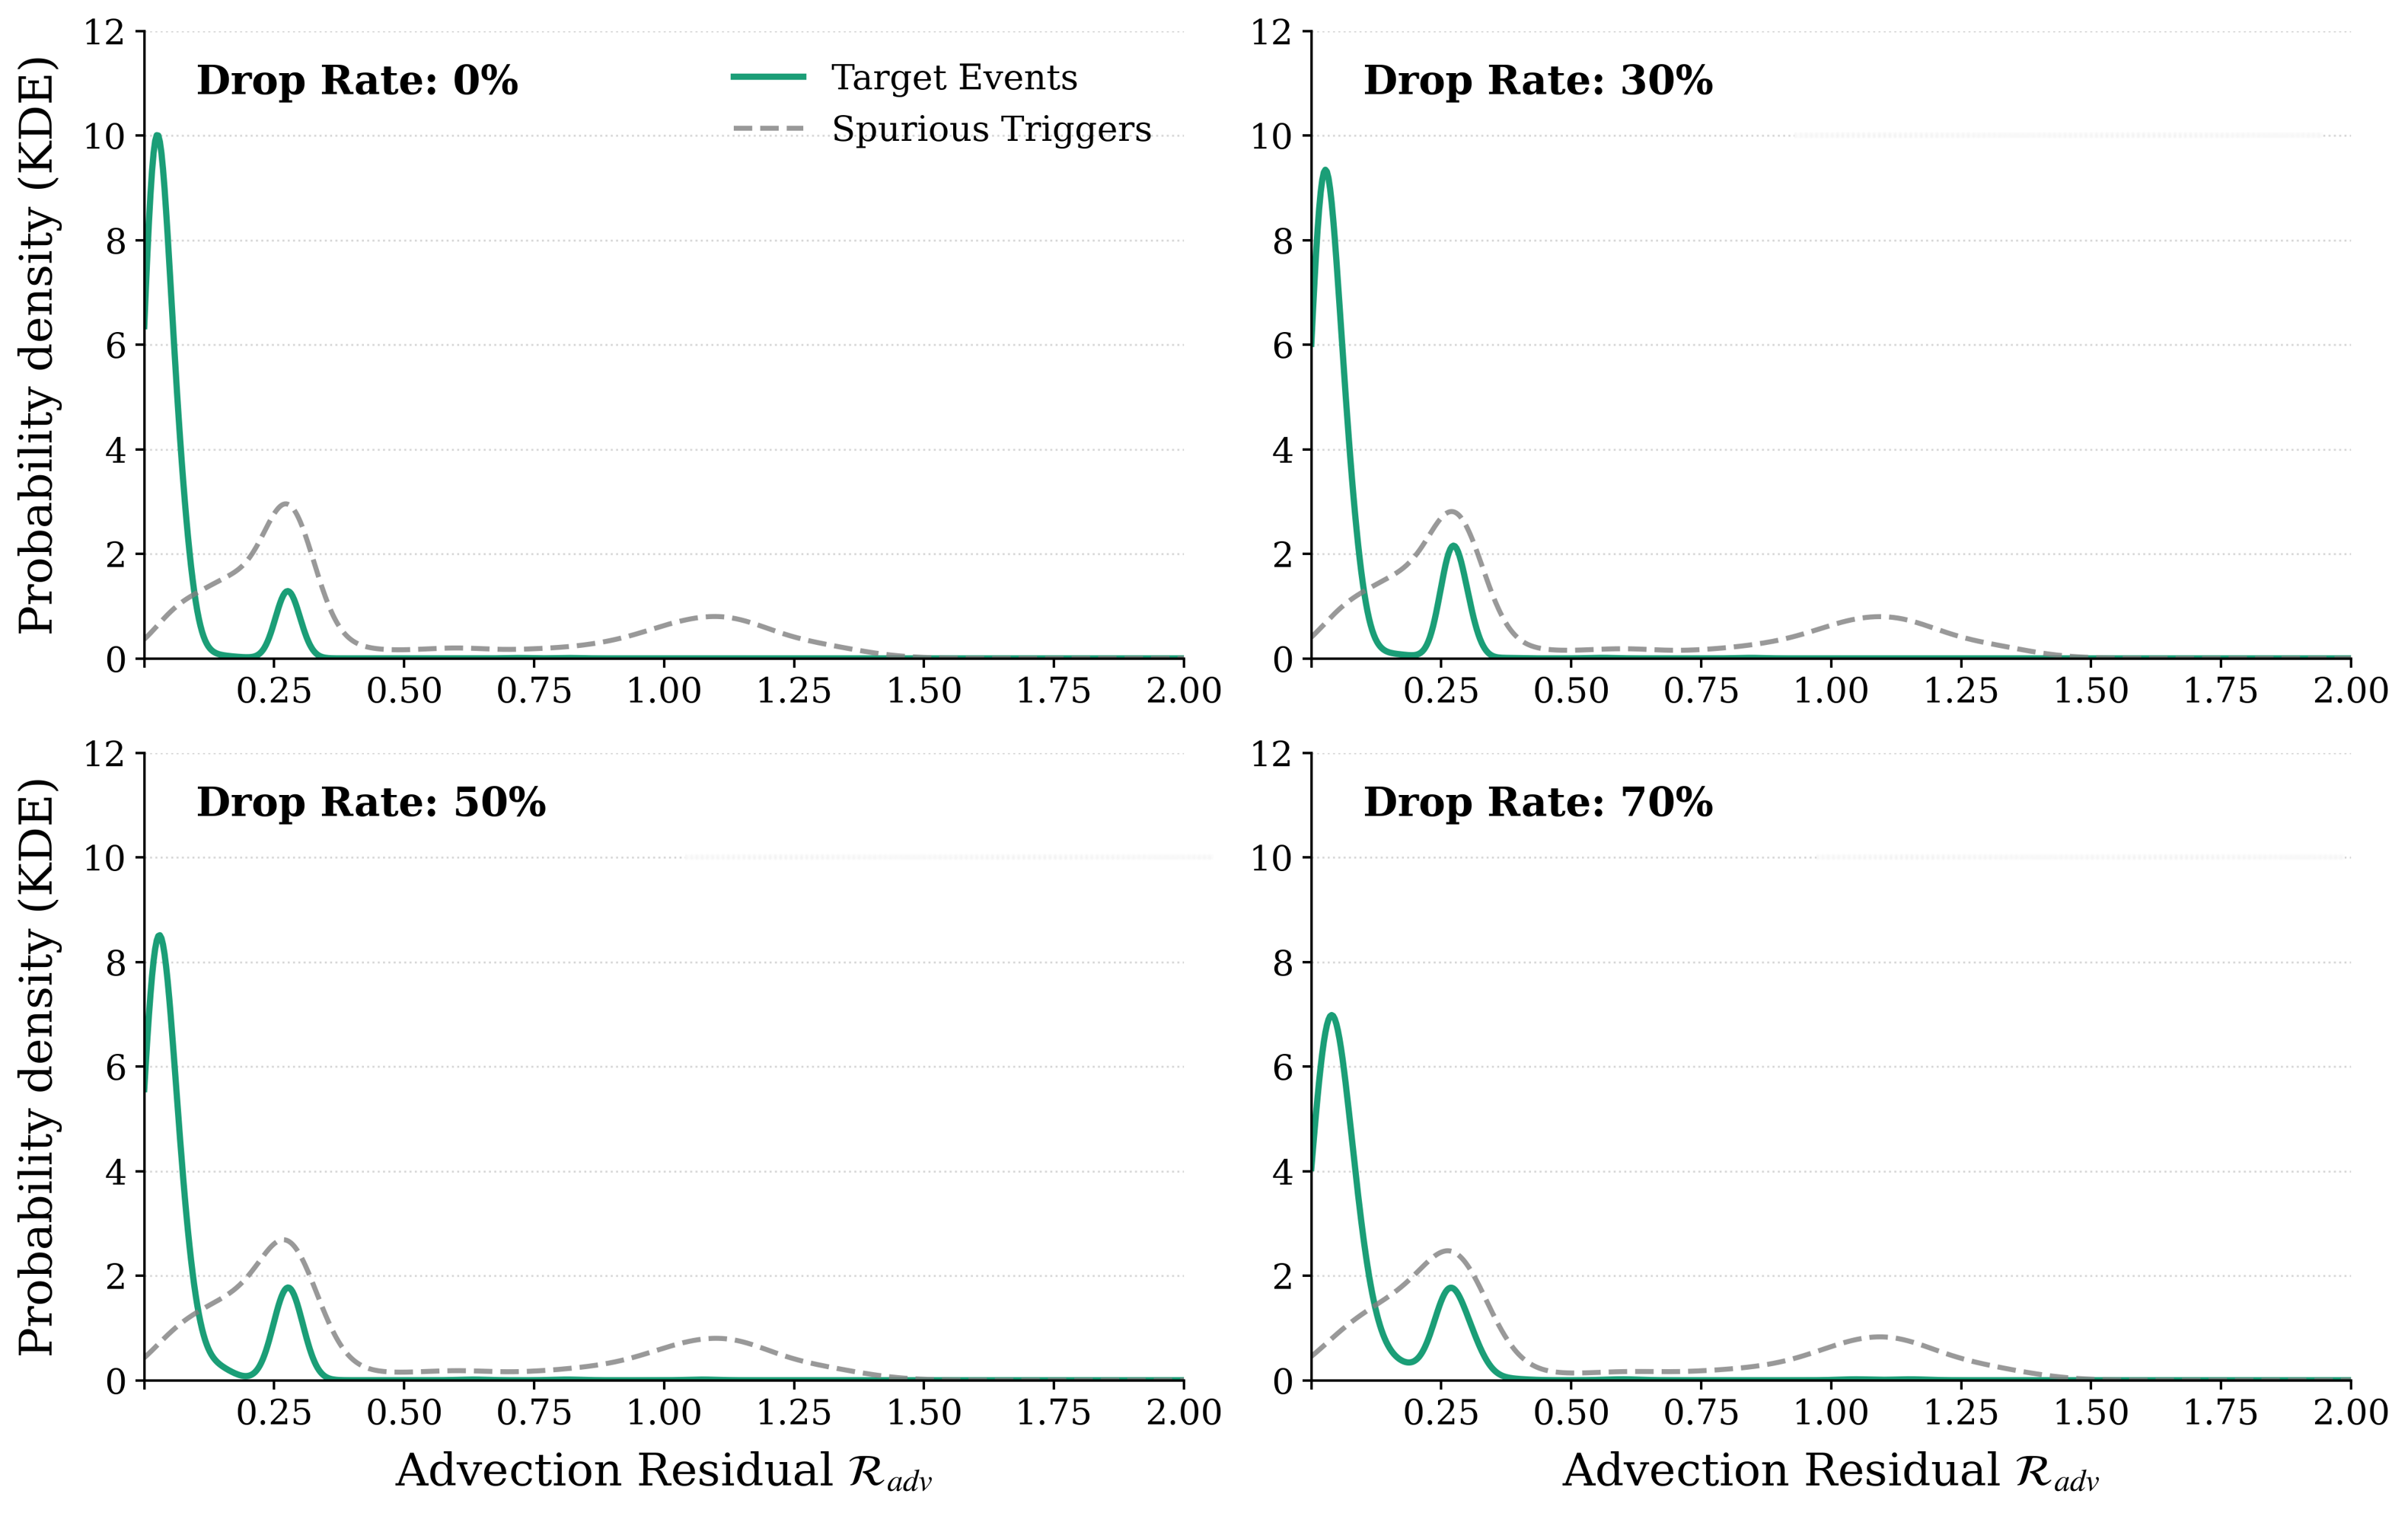
\includegraphics[width=\linewidth]{images/drop-exp.png}
  \caption{\textbf{Advection residual distributions under stochastic event dropping (0\%--70\%).}
  As sparsity increases, target events consistently maintain a sharp peak near zero, indicating that features are conserved along the predicted velocity field. 
  In contrast, spurious triggers exhibit much flatter and more dispersed residual distributions. 
  This suggests that PACT maintains temporal continuity through motion-consistent transport rather than relying on dense signal patterns.}
  \label{fig:robustness_kde}
\end{figure}

Across all drop rates, the residual distribution of target events consistently exhibits a pronounced peak near zero.
This indicates that, along the predicted velocity field, the transported features remain largely unchanged, despite substantial temporal gaps in the input stream.
Although the peak becomes slightly broader as the drop rate increases, its location remains stable even when up to $70\%$ of events are removed.
This behavior suggests that the model maintains feature continuity through motion-guided transport, rather than relying on dense temporal sampling.

In contrast, spurious triggers produce a much flatter and more dispersed residual distribution.
Since these events do not follow a coherent motion pattern, their features fail to satisfy the advection constraint, resulting in consistently higher residuals.
Importantly, the separation between the near-zero target peak and the noise distribution persists across all sparsity levels.

Taken together, these observations indicate that the robustness of PACT under extreme event dropping arises from the validity of its motion-consistent transport mechanism.
The model preserves feature coherence by propagating information along learned trajectories, instead of depending on repetitive or densely observed event patterns.


\bibliographystyle{splncs04}
\bibliography{main}

\end{document}